\documentclass[twocolumn, 12pt]{article}
\usepackage[utf8]{inputenc}
\usepackage{amsmath}
%\usepackage{marvosym}
\usepackage{textcomp}
\usepackage{geometry}
\usepackage{array}
\usepackage{wrapfig}
\usepackage{multirow}
\usepackage{graphicx}
\usepackage{float}
\usepackage{wrapfig}
\usepackage{caption}
\usepackage{amssymb}
\usepackage{ulem}
\usepackage[table]{xcolor}

\geometry{margin=.5in}

\begin{document}
\small


\section*{Heat Transfer Exam II}


\begin{equation*}
    \tau_s = \mu \left\frac{\partial u}{\partial y}\right|_{y=0}  \hspace{30pt} C_f = \frac{\tau_f}{\rho u_\infty^2 /2} (\text{local}) \hspace{30pt} Pr \triangleq \frac{\nu}{\alpha}
\end{equation*}
\begin{equation*}
    h \triangleq \frac{- k_f \left\frac{\partial T}{\partial y} \right|_{y=0} }{T_s-T_\infty} \hspace{10pt} \overline{h} \triangleq \frac{1}{A_s} \int_{A_s} hdA_s \hspace{10pt} \overline{h}_{\text{plate}} = \frac{1}{L} \int_{A_s} hdx 
\end{equation*}
\begin{equation*}
     Nu \triangleq \frac{hL}{k_f} = CRe_L^mPr^n \hspace{30pt} Nu \triangleq f(Re_L, Pr)
\end{equation*}
\begin{equation*}
    T_f = \frac{T_s + T_\infty}{2} \hspace{10pt} C_D = \frac{F_D}{A_f(\rho u^2/2)} \hspace{10pt} A_f \equiv \text{frontal area}
\end{equation*}




\subsection*{External Flow: Flat Plate}
\begin{equation*}
    \boxed{Re_{critical} = \rho \frac{u_\infty x}{\mu} = \frac{u_\infty x}{\nu} = 5\times10^5}
\end{equation*}
\begin{figure}[h]
    \centering
    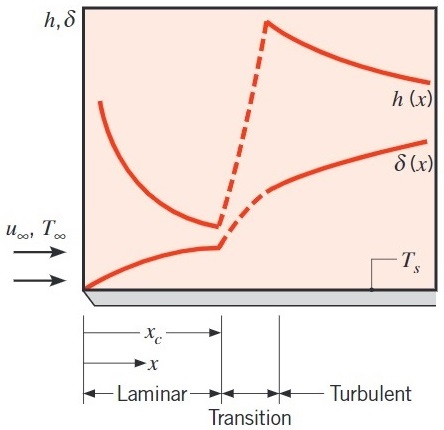
\includegraphics[scale=0.45]{h_and_delta_T_graphic.jpg}
    \label{fig:h_and_delta_T}
\end{figure}


\subsubsection*{Laminar Boundary Layer}
\begin{equation*}
    \delta = \frac{5x}{\sqrt{Re_x}} \hspace{30pt} C_{f,x} = \frac{\tau_x}{\rho u_\infty /2} = 0.664 Re_x^{-1/2}
\end{equation*}
\[
    Pr \geq 0.6 \Longrightarrow 
    \begin{cases}
        \frac{\delta}{\delta_T} \approx Pr^{1/3} \\
        Nu_x = \frac{h_x x}{k_f} = 0.332 Re_x^{1/2}Pr^{1/3}\\
        \overline{Nu}_x = \frac{\overline{h}_x x}{k_f} =0.664Re_x^{1/2} Pr^{1/3}
    \end{cases}
\]

\begin{equation*}
    \overline{C}_{f,x} = 2 C_{f,x} = 1.328Re_x^{-1/2}
\end{equation*}
\begin{equation*}
    Pe_x \triangleq Re_xPr
\end{equation*}
\[
    Pe_x \geq 100 \Rightarrow
    \begin{cases}
        Pr \leq 0.05  &\Rightarrow  Nu_x  = 0.564Pe_x^{1/2}\\
        \text{all } Pr  &\Rightarrow Nu_x = \frac{ 0.3387 Re_x^{1/2} Pr^{1/3}}{ [1 +(0.0468/Pr)^{2/3}]^{1/4}}
    \end{cases}
\]

\subsubsection*{Turbulent Boundary Layer}
\[
    Re_{x,crit} \leq Re_x \leq 10^8 \Longrightarrow
    \begin{cases}
        C_{f,x} = 0.0529 Re_x^{-1/5}\\
        \delta_T \approx \delta = 0.37xRe_x^{-1/5}
    \end{cases}
\]
\begin{equation*}
    0.6 \leq Pr \leq 60  \hspace{10pt} \Longrightarrow \hspace{10pt}Nu_x =0.0296 Re_x^{4/5}Pr^{1/3} 
\end{equation*}



\subsubsection*{Mixed Boundary Layer}
\begin{equation*}
    \overline{h}_L = \frac{1}{L} \left( \int_0^{x_c} h_{lam} dx +\int_{x_c}^L h_{turb}dx \right)
\end{equation*}
\begin{equation*}
    \overline{Nu}_L = (0.037 Re_L^{4/5} - A) Pr^{1/3}  \hspace{15pt} A  = 871
\end{equation*}
\[
    \Longrightarrow  \hspace{20pt}
    \begin{cases}
        0.6 \leq Pr \leq 60\\
        Re_x \leq Re_L \leq 10^8
    \end{cases}
\]



\subsection*{External Flow: Cylinder}
\begin{equation*}
    \boxed{ Re_{critical} = \rho \frac{u_\infty D}{\mu} = \frac{u_\infty D}{\nu} = 2\times 10^5  }
\end{equation*}
\begin{equation*}
    \theta_{lam} \approx 80 \deg \hspace{30pt} \theta_{turb} \approx 140 \deg
\end{equation*}
\begin{figure}[h]
    \centering
    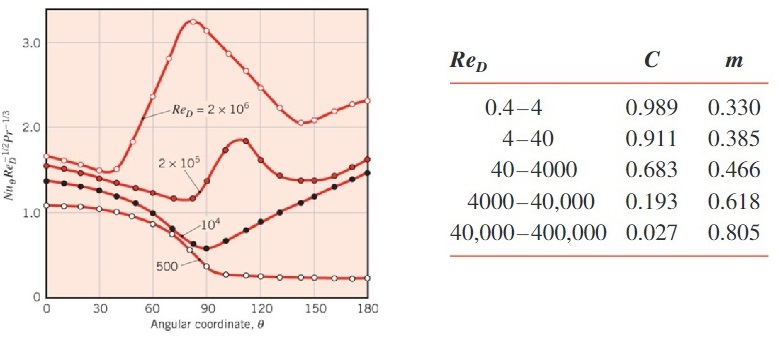
\includegraphics[scale=0.5]{NusseltSeperationAndTable7_2.jpg}
    \label{fig:NusseltVsSeperationAngleAndTable7_2}
\end{figure}
\begin{equation*}
    Pr\geq 0.7 \hspace{10pt} \Longrightarrow \hspace{10pt} \overline{Nu}_D = \frac{\overline{h} D }{k_f} = CRe_D^mPr^{1/3}  
\end{equation*}







\subsection*{External Flow: Sphere}
\begin{equation*}
    \boxed{ Re_{critical} = \rho \frac{u_\infty D}{\mu} = \frac{u_\infty D}{\nu} = 2\times 10^5  }
\end{equation*}
\begin{equation*}
    \overline{Nu}_D = 2 +(0.4Re_D^{1/2} + 0.06Re_D^{2/3}) Pr^{0.4} \left( \frac{\mu}{\mu_s} \right)^{1/4} = \frac{\overline{h} D}{k_f}
\end{equation*}
\[
\Longrightarrow \hspace{20pt}
\begin{cases}
    0.71 \leq Pr \leq 380\\
    3.5 \leq Re_D \leq 7.6 \times 10^4\\
    1.0 \leq \mu/\mu_s \leq 3.2\\
\end{cases}
\]
\noindent
All properties evaluated at \(T_\infty\), except \(\mu_s\) is at \(T_s\)



\subsection*{Internal Flow: Circular}
\begin{equation*}
    \boxed{ Re_{critical} = \rho \frac{u_m D}{\mu} = \frac{u_m D}{\nu} = 2300  }
\end{equation*}
\noindent
In fully developed region, \(u\neq f(x)\),  \(h \neq f(x)\) 
\begin{equation*}
    Re_D = \frac{4\Dot{m} }{\pi D\mu} \hspace{30pt} u_m \triangleq\frac{2}{r_o^2} \int_0^{r_o} u(r,x)rdr = \frac{\Dot{m}}{ \rho A_c}
\end{equation*}
\begin{equation*}
    \left(\frac{x_{fd,H}}{D} \right)_{lam} \approx 0.05Re_D \hspace{30pt} \left(\frac{x_{fd,H}}{D} \right)_{turb} \approx 10
\end{equation*}
\begin{equation*}
    \left(\frac{x_{fd,T}}{D} \right)_{lam} \approx 0.05Re_DPr \hspace{30pt} \left(\frac{x_{fd,T}}{D} \right)_{turb} \approx 10
\end{equation*}
\begin{equation*}
    u(r) = \frac{1}{4\mu} \left(\frac{dP}{dx} \right)r_o^2 \left[1-\left(\frac{r}{r_o} \right)^2 \right]
\end{equation*}
\begin{equation*}
    \frac{u(r)}{u_m} = 2\left[1-\left(\frac{r}{r_o} \right)^2 \right]
\end{equation*}
\begin{equation*}
    q =\Dot{m}c_p(T_{m,o} - T_{m,i}) = \overline{h} A_s (T_s-T_m)
\end{equation*}
\begin{equation*}
    T_m = \frac{2}{u_mr_o^2} \int^{r_o}_0 uTrdr \hspace{30pt} \overline{T}_m =\frac{T_{m,i} +T_{m,o}}{2}
\end{equation*}
\begin{equation*}
    \frac{dT_m}{dx} = \frac{P}{\Dot{m}c_p} q_s'' = \frac{P}{\Dot{m}c_p} h (T_s-T_m)
\end{equation*}


\subsubsection*{Reynolds Number}
\textbf{if \(Re_D \leq 2300\),}
    \[
        \text{eval  @ } \overline{T}_m \Rightarrow
        \begin{cases}
            q_s'' = \text{const} \hspace{5pt} \Rightarrow \hspace{5pt} Nu_D =\frac{hD}{k_f} = 4.36\\
            T_s =\text{const} \hspace{5pt} \Rightarrow \hspace{5pt} Nu_D =\frac{hD}{k_f} = 3.66
        \end{cases}
    \]
    \noindent
        \textbf{else}
        \[
            Nu_D = 0.23Re_D^{4/5}Pr^n \hspace{7.5pt} \Longrightarrow \hspace{7.5pt} 
            \begin{cases}
                n = 0.4 &T_s>T_m\\
                n=0.3 &T_s<T_m
            \end{cases}
        \]
        \[
            \Longrightarrow \hspace{20pt}
            \begin{cases}
                0.6 \leq &Pr \leq 160\\
                        &Re_D \geq 10,000\\
                        &L/D\geq 10\\
            \end{cases}
        \]


\subsubsection*{Constant Uniform \(q_s''\)}
\begin{equation*}
    q_{conv} = q_s ''PL  \hspace{30pt} T_m(x) = T_{m,i} + \frac{P}{\Dot{m}c_p} q_s ''x
\end{equation*}





\subsubsection*{Constant Uniform \(T_s\)}
\begin{equation*}
    q_{conv} =\Dot{m}c_p(T_{m,o} - T_{m,i}) = \Dot{m}c_p (\Delta T_i - \Delta T_o)
\end{equation*}
\begin{equation*}
    \Delta T_i \triangleq T_s - T_{m,i} \hspace{30pt} \Delta T_o \triangleq T_s - T_{m,o}
\end{equation*}
\begin{equation*}
    \Delta T_{lm} \triangleq \frac{\Delta T_o -\Delta T_i} {ln(\Delta T_o/ \Delta T_i)} \hspace{30pt} q_{conv} = \overline{h}A_s \Delta T_{lm}
\end{equation*}
\subsubsection*{Constant Uniform \(T_\infty\)}
\begin{equation*}
    \frac{\Delta T_o}{\Delta T_i} = \frac{T_\infty - T_{m,o}} {T_\infty -T_{m,i}} = exp\left( - \frac{\overline{U}A_s}{\Dot{m} c_p}\right) 
\end{equation*}
\begin{equation*}
    \overline{U}A_s = \frac{1}{R_{tot}} \hspace{30pt} q_{conv} = \overline{U} A_s \Delta T_{lm}
\end{equation*}



\subsection*{Internal Flow: Non-Circular}
\begin{equation*}
    T_m = \frac{1}{\Dot{m}c_p} \int_{A_c} \rho Uc_p TdA_c 
\end{equation*}
\begin{equation*}
    D_h = \frac{4A_c}{P} \hspace{30pt} Re_D = \frac{\rho u_mD_h}{\mu }
\end{equation*}
\noindent
\textbf{if \(Re_D \leq 2300\),}
\begin{figure}[H]
    \centering
    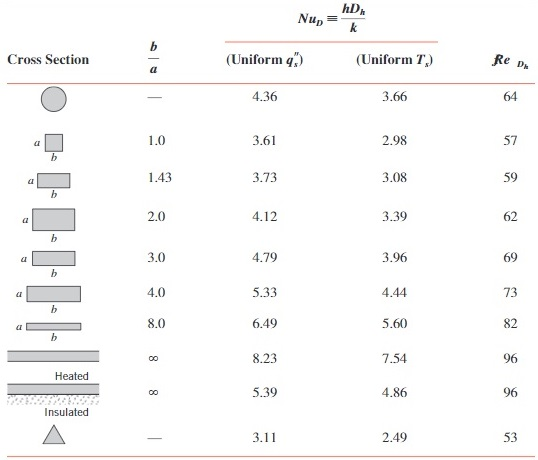
\includegraphics[scale=0.7]{Table8_1.jpg}
    \label{fig:Table8_1}
\end{figure}

\noindent
\textbf{else}\\

Use the correlation listed under the Reynolds Number subsection.

\vspace{110pt}
\subsection*{Locations of Appendices and Tables}
    \begin{tabular}{|l|l|l|}
        \hline
        \rowcolor{lightgray}
        Fin Temp table & Table 3.4 & pg 161 \\
        \hline
        Finite Diff. Equations & Table 4.2 & pg 246\\
        \hline
        \rowcolor{lightgray}
        Spatial Effects Coeff. & Table 5.1 & pg 301 \\
        \hline
        Dimensionless Params & Table 6.2 & pg 408\\
        \hline
        \rowcolor{lightgray}
        Cylinder in Cross Flow & Table 7.2-7.3 & pg 458\\
        \hline
        Non-Circular Tubes & Table 8.1 & pg 553\\
        \hline
        \rowcolor{lightgray}
        Fouling Factors & Table 11.1-11.2 & pg 709\\
        \hline
        NTU Effectiveness & Table 11.3-11.4 & pg 724\\
        \hline
        \rowcolor{lightgray}
        Fractional Blackbody & Table 12.2 & pg 786\\
        \hline
        Thermophysical props. & Appendix A & pg 981\\
        \hline
        \rowcolor{lightgray}
        Zeta values for \(\zeta_1 - \zeta_4\) & Appendix B.3 & pg 1016\\
        \hline 
        Bessel Functions  & Appendix B.4 & pg 1017\\
        \hline 
        \rowcolor{lightgray}
        Heat generation eq's & Appendix C & pg 1019\\
        \hline
        Turbulent BL & Appendix F & pg 1032\\
        \hline
           
    \end{tabular}

\end{document}